\documentclass{article}
\usepackage[utf8]{inputenc}
\usepackage[english]{babel}
\usepackage[font=small,labelfont=bf]{caption}
\usepackage{geometry}
\usepackage{natbib}
\usepackage{pxfonts}
\usepackage{graphicx}
% \usepackage{amsmath}
% \newcommand{\rpm}{\raisebox{.2ex}{$\scriptstyle\pm$}}
% \DeclareMathOperator*{\argmax}{arg\,max}
\usepackage{newfloat}
\DeclareFloatingEnvironment[name={Supplementary Figure},fileext=lof]{suppfigure}

\title{Capturing the shape of our experiences and how we remember them}
\author{Andrew C. Heusser \& Jeremy R. Manning}
% \affiliation{Dartmouth College}

\bibliographystyle{apa}

\begin{document}
\maketitle

\section{Abstract}
{
The human memory system is adept at cataloging the rich dynamics of ongoing experience. A defining feature of our everyday experiences is that they unfold in a structured and predictable manner. This temporal structure gives each of our experiences (and thus our memories for those experiences) a unique shape.  However, temporal structure is typically absent (or severly impoverished) in traditional trial-based memory experiments. As a consequence, our understanding of how the temporal structure (i.e. the shape) of our experiences influences memorability and memory organization is limited. In this study, we investigate how people verbally recount a video by characterizing and relating the thematic dynamics, or ``trajectories,'' of the stimulus and participants' recalls. Using a novel approach based on topic modelling, we found that despite substantial variability in the quantity of information recalled across participants as well as the particular words used to describe the experience, the overall shape of the stimulus was recapitulated by most of the participants. These findings provide a window into which aspects of naturalistic experiences must be preserved, and which might be more flexible, in considering whether and how those experiences are remembered.

\section{Introduction}

What does it mean to \textit{remember} something? In traditional episodic memory experiments \citep[e.g., list-learning or trial-based experiments;][]{Murd62a, Kaha96}, remembering is often cast as a binary operation: either an item is recalled or it isn't. More nuanced studies might incorporate self-reported confidence measures as a proxy for memory strength, or ask participants to discriminate between ``recollecting'' an experience or a feeling of ``familiarity'' \citep{Yone02}. However, characterizing and evaluating memory in more realistic contexts (e.g., telling a story to a friend about a movie you recently saw) is much more nuanced. Real-world recall is continuous, rather than binary.  The specific words used to describe an experience have very little bearing on whether the experience is considered to have been ``remembered.''  Further, one might remember the gist of an experience but forget (or neglect to recount) particular details.  Or different people who share an experience might recount the experience with a similar level of detail, but the specific details that were remembered might vary across people.  Which aspects of those recollections should be considered fundamental, and which are extraneous to the main story?

Human memory studies typically assess memory for the elements within an experience, such as the people, places and things encountered. However, real life experiences can also be described in terms of their temporal structure (i.e. how the contents relate/change over time).  For instance, naturalistic experiences are autocorrelated in space and time on short timescales. In other words, the contents of an experience are often similar from moment to moment and change gradually. As an example, many of us spend our mornings/evenings at home and much of our days at work (e.g. an office). While the specific happenings within these contexts differ, they are often highly correlated (and thus predictable) over time. Furthermore, our experiences can also be characterized by longer timescale correlations. For example, consider returning to your office after taking a lunch break. The spatial contexts before and after lunch are highly similar, but separated in time. Thus, while evaluating the ability to recall the isolated elements of an experience has been a fruitful way to learn about human memory, another important dimension to consider is the temporal structure of the remembered experience, and how the temporal structure of the memory relates to the original experience. However, these recurrent and gradually changing temporal dynamics are not typically present in traditional memory studies, but are likely critical if we wish to understand how our memory systems remember our life experiences.

While our experiences often change gradually, they can also change rapidly (e.g. walking through a doorway) \citep{RadvZack17}. Prior research suggests that these sharp transitions (coined in the literature as ``event boundaries'') during an experience may serve to descretize our memories into ``events'' \citep{RadvZack17, BrunEtal18, HeusEtal18, ClewDava17}. Short timescale autocorrelations in the contents of an experience are thought associatively link information in memory, while more drastic changes in perceptual or semantic aspects of an experience may lead to discontinuities in memory \citep{HeusEtal18, BrunEtal18}.  In other words, the interplay between stable and transient temporal dynamics may impose structure on memories for those experiences. There is now compelling evidence that event boundaries can influence memory organization when learning sequences of items \citep{HeusEtal18, DuBrDava13}, during navigation \citep{BrunEtal18}, and narrative comprehension \citep{ZwaaRadv98, EzzyDava11}.  However, whether people verbally recount their experiences in a way that is structured around events has not been established.

In this study, we analyzed an open dataset in which participants view and then verbally recall an episode of the BBC series \textit{Sherlock} \citep{ChenEtal17}. To capture the temporal structure of the video, we developed a novel computational approach based on topic modeling \citep{BleiEtal03} and hidden Markov models \citep{Rabi89, BaldEtal17}. This model casts naturalistic stimuli as high-dimensional topic ``trajectories'', whereby the theme of each moment of the video is represented as a topic vector. In this framework, successful remembering entails verbally ``traversing'' the path formed by the stimulus topic trajectory as closely as possible. We hypothesized that successful memory for a naturalistic stimulus is given by a recall trajectory that closely follows the path (and covers the entirety) of the stimulus trajectory.

\subsection{Results}

\begin{figure}[th!]
\centering
\includegraphics[width=1\textwidth]{figs/1_analysis_schematic.pdf}
\caption{\small \textbf{Schematic of the analysis approach.} For each scene in the video, text descriptions were generated by hand. Three exemplary time points are displayed here.  Below the video descriptions are text samples from an example participant's verbal recall transcript.  We fit a topic model to the moment-by-moment video text descriptions and transformed participant's verbal recall transcripts using this same model. The bar charts display the resulting topic model weights for the video (in blue) and recall (in orange) for three example topic dimensions.}
\label{fig:schematic}
\end{figure}

\subsubsection{Modeling the naturalistic stimulus and verbal recall}
We fit a topic model \citep{BleiEtal03} to hand-annotated text descriptions of scenes from the video. The text descriptions contained details of the scene such as the characters, location, and a short summary of the scene (see Fig.~\ref{fig:schematic} for example text, see Methods for analysis details). As depicted in Fig.~\ref{fig:model}a, the topic vectors are sparse and change slowly over time. Furthermore, there are clear transitions from one topic ``state'' to the next, possibly indexing scene transitions in the stimulus. To get a better handle on this temporal structure, we computed a timepoints (1976) by timepoints (1976) correlation matrix of the video model (Fig.~\ref{fig:model}c).  This correlation matrix reveals that the model has a strong, block-diagonal structure with very low off-diagonal correlation values, suggesting the representations of each block are unique and highly descriminable.

After watching the video, participants verbally recalled (in order) as much of the episode as they could.  We used the same topic model (fit with the text descriptions of the video) to transform participants' verbal recall transcripts. An example participant's (\#13) recall model is plotted in Fig.~\ref{fig:model}b. Like the video model, topic vectors were sparse and changed gradually.  Then, we investigated the temporal structure of the recall matrices. From each participant's recall model, we computed a timepoint (68 to 294) by timepoints by timepoints (range: 68 to 294) correlation matrix. An example participant's (\#13) correlation matrix is plotted in Fig.~\ref{fig:model}d. Like the video model, each participant's recall correlation matrix exhibited a strong block-diagonal structure (Supp. Fig.~\ref{fig:corrmats}). Notably, this suggests that participants recounted the video in discriminable segments, likely related to the recall of specific events from the video.


\begin{figure}[ht!]
\centering
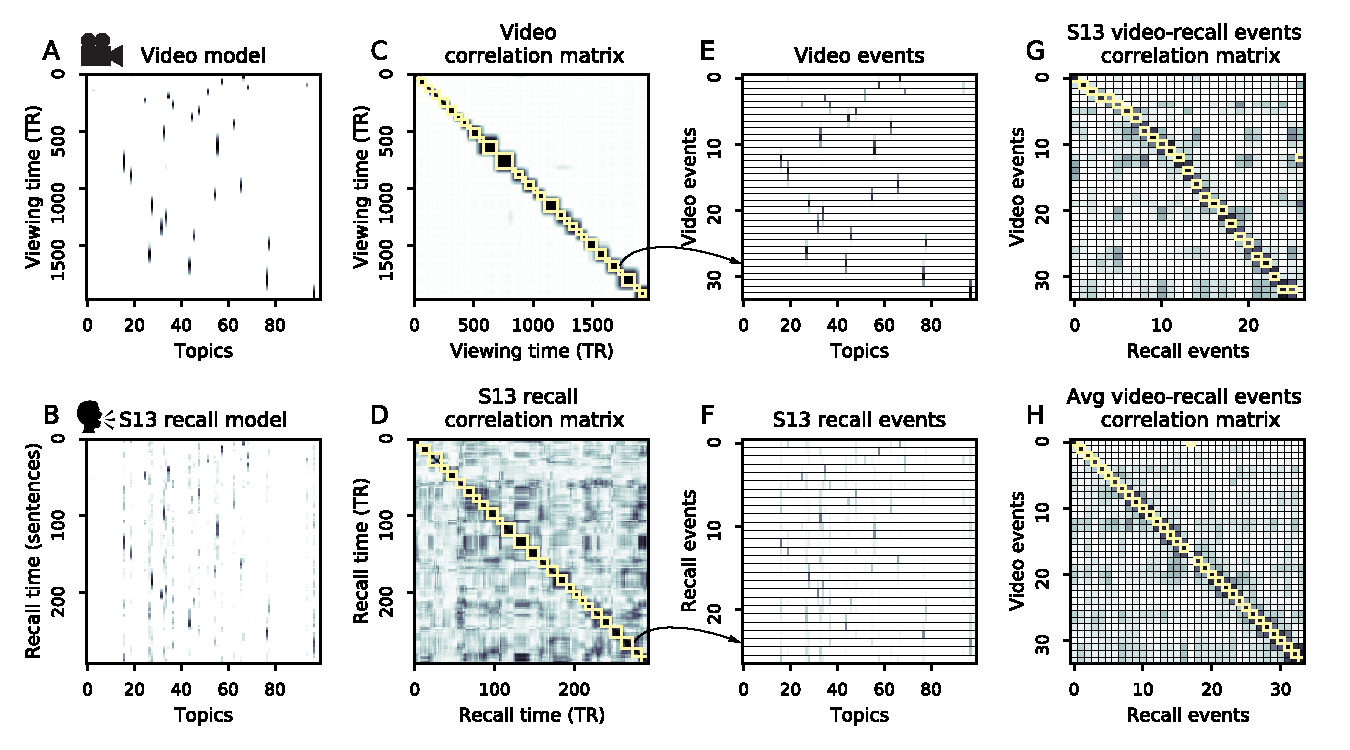
\includegraphics[width=\textwidth]{figs/2_eventseg.pdf}
\caption{\small \textbf{Modelling naturalistic stimuli and recall.} A depiction of our analysis pipeline. For all plots, darker colors indicate greater values and the range of each plot is 0-1.  A). A timepoints (1976) by topics (100) matrix representing the video stimulus.  Each row represents the most likely mixture of topics for a given timepoint (i.e. topic weights). Each column represents a different topic. B). A timepoints (1976) by topics (100) matrix representing participant \#13's recall. C). A viewing-time (1976) by viewing-time (1976) correlation matrix representing the correlation of each moment of the video model with every other moment of the video model. The white boxes represent `events' recovered by a hidden Markov model. D). A recall-time (294 sentences) by recall-time (294) correlation matrix for participant \#13. E). An events (34) by topics (100) matrix where each row represents the average topic vector for each event in the video model.  F). An events (27) by topics (100) matrix where each row represents the average topic vector for each event in participant \#13's recall model. G. A recall events (27) by video events (34) correlation matrix for participant \#13. The cells with a yellow border identify the video event with the highest correlation to a given recall event. F. A group averaged recall events (34) by video events (34) correlation matrix.  The cells with yellow borders are the video event with the highest correlation to a given average recall event.}
\label{fig:model}
\end{figure}

\subsubsection{Segmenting the video and recall models into ``events''}
As described above, a striking feature of both the video and recall correlation matrices is a strong, block structure along the diagonal of the matrices (see Fig.~\ref{fig:model}c,d).  We hypothesized that this structure might arise from transient stability in the "theme" of both the video and of participants' memory for the video. We hypothesized that specific events described by a participant could be ``matched'' to specific video events by computing the similarity (i.e. correlation) between their topic vectors. In other words, the video event that is most similar to a particular recall event is the event that the participant is most likely describing. To test this idea, we segmented the video and recall models in $k$ events (i.e. states) using a hidden Markov model ~\citep{BaldEtal17}. Our algorithm determined 34 events for the video model and a range of values (range: 8-27; mean: 15.41; SD: 5.6) for the recall models (see Methods for details on choosing an optimal $k$ value).  The events discovered for the video model and a representative participant's recall model are highlighted as yellow rectangles outlining blocks along the diagonal of the correlation matrices (Fig.~\ref{fig:model}b,d).

Next, we created a video ``event model'' by averaging together neighboring topic vectors that the were classified to be in the same event, resulting in an events (34) by topics (100) matrix (Fig.~\ref{fig:model}e).  We performed the same procedure for the recall matrices (Fig.~\ref{fig:model}f). Then, we computed the correlation between video and recall event models, resulting in a video events (34) by recall events (8-27, depending on the participant) correlation matrix (Fig~\ref{fig:model}g for example, Supp. Fig~\ref{fig:matchmats} for all participants). These matrices represent the similarity (correlation) between each video event and each recall event (for each participant). To determine which video event a particular recall event was most likely describing, we computed the index of the video event with the highest correlation to the recall event (i.e. the argmax).  This is depicted in Fig.~\ref{fig:model}g as the cells highlighted with a yellow border. Notably, our algorithm suggests that the example participant recalled most of the video events and did so in order.

Then, we computed a group-averaged recall event model and video-recall event correlation matrix. For each participant (and each recall event), we sorted the recall event vectors (across all participants) according to the video event with the highest correlation. We then averaged the recall event vectors within each group. This yielded an average recall event vector for all but one (of 34) video events, since no participant remembered one of the events according to our model. Lastly, we computed an average recall event (34) by video event (34) correlation matrix, and highlighted the cell with the highest correlation value with a yellow border (Fig.~\ref{fig:model}h). Notably, this matrix displayed high correlation values along the diagonal and low correlations in the off-diagonal cells. This suggests that on average, participants were able to recapitulate the events in the episode in a specific and highly descriminable way.

\subsubsection{The shape of a naturalistic experience is preserved in recall}
Classic approaches to studying free recall in episodic memory (such as overall accuracy and serial position curve) focus on the quantity of information recalled \citep{Murd62a}. More recent metrics (such as lag-CRP, semantic and temporal clustering) go further to describe list-level memory organization \citep{Kaha96, PolyEtal09}. However, these approaches cannot (and were not designed to) capture the rich temporal dynamics inherent in naturalistic stimuli and associated recall of those experiences. In the next set of analyses, we test the hypothesis that successful recall of a naturalistic stimulus entails recovering the trajectory of a stimulus.

\begin{figure}[t!]
\centering
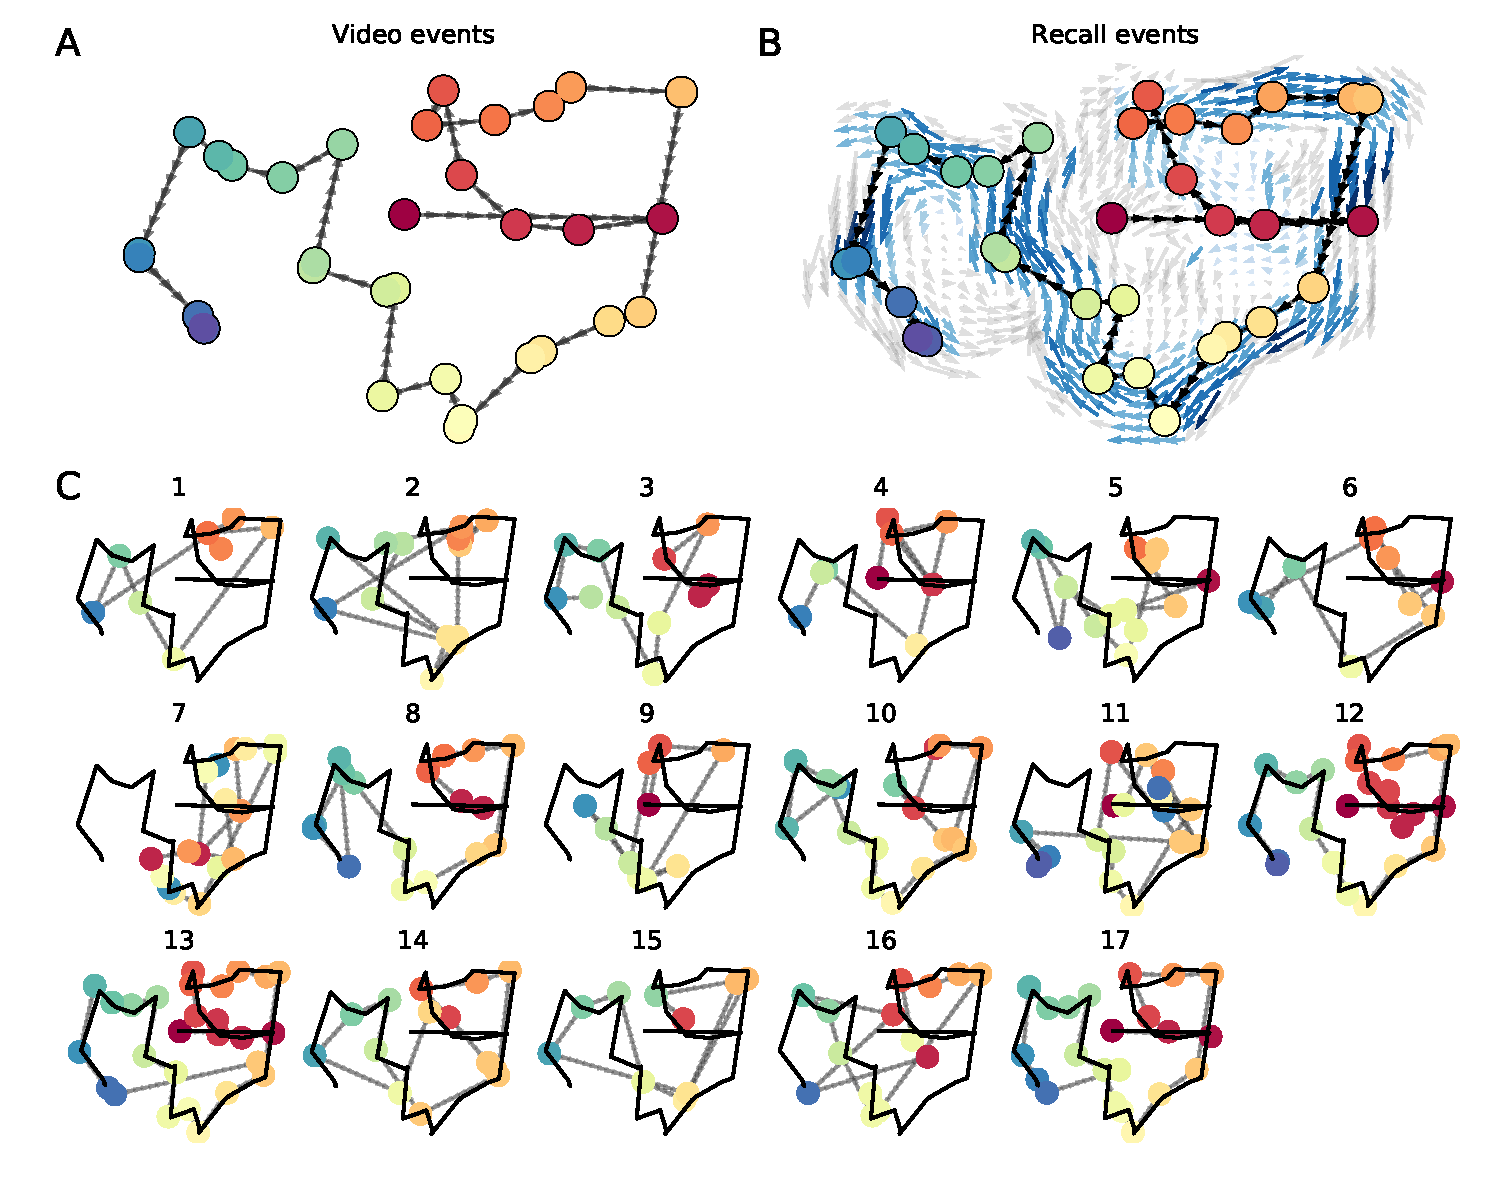
\includegraphics[width=1\textwidth]{figs/3_trajectory.pdf}
\caption{\small \textbf{Video and recall trajectory plots.} A). 2-dimensional embedding of the video events model (reduced with UMAP algorithm). The arrows indicate the forward direction of the video events. B). 2-dimensional embedding of the average recall events model.  The colors refer to the most similar video events. The directional lines connecting the points represent the true video event order. The arrows represent the group-average direction of all recall event transitions (i.e. a line segment connecting two consecutive recall event vectors) that intersected a box (width=.25) centered on the origin of the arrow.}
\label{fig:trajectory}
\end{figure}

To visualize the relationship between the video and recall event models, we embedded them into a 2D space using the UMAP dimensionality reduction algorithm ~\citep{McInHeal18}, where the points represent video/recall events and the distance between them represents their similarity/distance in ``topic space'' (Fig.~\ref{fig:trajectory}a).  We observed that visually, it appears that the two models have a very similar temporal evolution and geometric structure. To further quantify this correspondence and to characterize how participants navigated through the space during recall, we analyzed the angle between successive recall events. We created a grid of evenly spaced points (.25 units) in the 2D ``topic space''. For each point on the grid, we drew a circle (radius=.25) around the point and grouped together all recall transitions that intersected the circle (across subjects). To visualize the average angle, we converted each transition angle to a unit vector and then averaged the vectors together. To assess consistency in the direction of the recall transition across participants, we performed a Rayleigh test (p$<$.001, corrected at p$<$.05 using permutation procedure described in Methods). Notably, all video events fell within the path formed by the video events.  Thus, participants' recalls followed the same path as the video model (Fig.~\ref{fig:trajectory}b), suggesting the shape of the stimulus was preserved despite idiosyncratic differences between participants in their recalls.

%NOTE: it feels like we need some more supporting evidence that the shape of the video and the recall trajectories are related.  one possibility would be to add the analysis where i compute the distance between each recall event and the line formed by each video transition per subject. the result is that hand annotated memory correlates to this distance, suggesting that subjects who better capture the shape also have better memory on average.

\begin{figure}[t!]
\centering
\includegraphics[width=1\textwidth]{figs/4_topics.pdf}
\caption{\small \textbf{Analysis of topics by event memorability.} A). Group-averaged correlation between each video event and closest recall event (per subject). Error bars represent 95\% confidence intervals. B). Wordles (top 200 words) representing a weighted average of video event topic vectors weighted by event memorability (e.g. the correlation values in A). The top wordle (green) contains words from the most remembered events and the bottom (red) contains words from least memorable events. The word sizes are proportional to the word's ``activation''. C). Trajectory represents the video event model embedded in a 2D space using UMAP. The large colored dots are video events. The small colored dots are all individual recall events across all participants, where the colors refer to the closest video event. The circular wordles represent the top 3 most (green circles) and least (red) memorable video events.  The left side of the wordle circles contain words associated with the video event vector and the right side contains words associated with the average recall event vector.}
\label{fig:topics}
\end{figure}

\subsubsection{Memorability by event and topics}
A notable advantage of representing naturalistic stimuli/memory using this approach is that the event models can be mapped back to the language used to fit the model(s).  This allows for analysis (and visualization) of the language used when participants' recounted their experiences.  In this next analysis, we 1) quantified the memorability of each video event and 2) used memorability to plot the top words for the most and least memorable scenes.

To measure video event memorability, we computed the correlation between each video event and the closest recall event and then averaged those values within participant (Fig.~\ref{fig:topics}a). We used event memorability to create a weighted average over all video event vectors, where video events with better memory were weighted more heavily. Then, we extracted the top 200 words and created ``wordles'' representing the most memorable themes in the video. The results reveal that scenes containing ``Sherlock'' and ``John'' were highly memorable, and also scenes containing words such as ``medium'', ``street'' and ``baker'' (Fig.~\ref{fig:topics}b). To find words related to the least memorable scenes, we inverted the memorability weights and again extracted the top 200 words.  Scenes containing ``Mike'' and ``Molly'' were least remembered, and also words like ``conference'', ``hospital'' and ``psychotherapist'' (Fig.~\ref{fig:topics}b).

Then, we took a closer look at the themes contained in the top/bottom 3 events, using the memorability weights to select the top/bottom events. We performed the same analysis as described above, but separately for the video and average recall event vectors representing each of the top/bottom 3 remembered events. In Figure~\ref{fig:topics}c, the trajectory represents a low-dimensional embedding of the video model and the large colored dots represent the video events. The smaller colored dots represent the distribution of individual recall events across all participants, colored by the closest video event. We plotted wordles for the top 3 (circled in green) and bottom 3 (red) most/least remembered events, where the video is represented in the left half of the circle and the average recall is represented in the right half of the circle. Visual inspection reveals that the words contained in the memorability weighted worldles (Fig.~\ref{fig:topics}b) overlap with the individual top/bottom event wordles (Fig.~\ref{fig:topics}c). These analyses shed light on the contents of naturalistic stimuli and accompanying memories, and highlight the flexibility in transforming between human and machine readable representations of the data afforded by our modeling approach.

\subsubsection{Additional measures of naturalistic recall}
Representing the video and verbal recall as events in ``topic space'' also affords us the ability to characterize the quality of recall in a more fine-grained and nuanced way than what was previously possible. We quantified the distance between each video event and its matching recall event (``precision''), the the distance between a video event and all non-matching recall events (``distinctiveness'') and the temporal order of the recall events (``order''). All three of these metrics were correlated to hand-annotated memory performance across participants (p$<$.05, see Supplemental Materials Section 1 for details).

Just like in a traditional ``free-recall'' list-learning experiment where participants view a list of words and then verbally recall them, our video-recall matching analysis approach affords us the ability to analyze memory in the same way. We considered 6 classic list-learning analyses: overall accuracy, probability of first recall \citep{Hoga75, HowaKaha99, Lami99}, lag-conditional response probability \citep{Kaha96, HowaKaha99}, serial position curve \citep{Murd62a}, temporal clustering and semantic clustering \citep{HowaKaha02, PolyEtal09}. Extending these classic list-learning analyses to naturalistic stimuli allows to directly compare trial- and naturalistic-based recall studies (see Supplemental Materials Section 2 for details).

\section{Discussion}
\label{sec:discussion}
Studying human memory is commonly distilled down to a process of matching specific moments of a past experience with specific mnemonic outcomes.  In traditional trial-based free recall experiments, individual stimuli encountered during encoding are typically labeled as ``remembered'' or ``forgotten'' depending on whether the stimulus is recalled/recognized during a subsequent test. While this approach has advanced our understanding of human memory immensely, it does not translate well to naturalistic experiences. For one thing, the contents of our recall at any given moment might be reflected in many prior experiences/moments. Furthermore, the particular words used to describe the experience will inevitably vary across people and even across repeated recollections within an individual. Thus, there is not a ``one-to-one'' mapping between naturalistic experiences and their mnemonic counterparts. For example, remembering the patterns and colors of each person's shirt in a crowd might be considered as excellent recall in a standard memory task setup. But if the rememberer failed to note that the people in the crowd were gathered for their surprise birthday party, then they would have missed the "point" of the experience.

Our topic modeling approach, whereby we consider the broad ``theme'' present in different moments of participants' experiences and their memories for those experiences, affords us the ability to flexibly and accurately characterize memory for naturalistic experiences. This approach allows us to quantify which moments from the past and the current recounted experience match in terms of their thematic content and critically, our ability to perform this matching does not require participants to use any specific overlapping words. Our work characterizes experience by comparing the overall ``shape'' of a dynamic stimulus and a memory. We assess the quality of memory for the movie participants viewed by measuring the match between the shapes of the movie's trajectory and each participant's recall trajectory. By contrast, the number of recalls could be captured by the "sampling frequency" along that trajectory-- but the number of recalls alone cannot tell us whether participants successfully recollected the meaning of the story by capturing the salient points of the narrative that define its main shape.

In addition to providing a way to capture the shape of an experience, this method affords the ability to quantify the particular contents of memory.  Whereas traditional approaches abstract over the content (e.g. percent correct), Our approach allows one to quantify which aspects of an experience are memorable and which fail to stick. This aspect of our approach opens the door for a much richer characterization of memory that considers not just how much information was recalled, but the particular details of that information as well.

More broadly, these findings have strong implications for how we assess memory in other naturalistic contexts, such as the classroom or in a doctor's office.  Whereas tests often measure students' performance using metrics such as the proportion of correctly answered questions, our work suggests that this approach might miss the ``forrest for the trees''. We view ``true learning'' as understanding the key concepts (i.e. understanding key themes in the learned content and how they relate) rather than about regurgitating the greatest number of facts. In addition to educational contexts, our approach may provide unique metrics that can be used to assist in the diagnosis of a memory disorder, and other psychiatric disorders that influence memory. For example, while the quantity of information recalled could be roughly matched between a healthy and patient population, other aspects of the memory (such as the shape, serial order, precision or distinctiveness) might be different. Thus, this work serves as a foundation for more nuanced approaches to memory assessment that consider the trajectory and specific contents of memory for a naturalistic experience.

An important question for future work concerns the factors that drive an individual to sample their recall trajectory finely or coarsely. For example, given a short recall interval, would participants intuitively gravitate towards coarser samplings that still outline the basic shape of the movie's topic trajectory? Or if participants were told that their narrations would be played back to other participants ~\citep{ZadbEtal16}, would that change the resolution or shape of their recalls? And over successive recountings of the same sequence of events or with more elapsed time between encoding and recall, how do the shapes of the trajectories change? For example, loss of detail would result in a "smoothing out" of the trajectories with each new retelling.

While we view this work as a major advance in characterizing and understanding human memory, as with any approach there are limitations. First, the approach relies on having a ``good'' model of the stimulus (e.g. one that describes the video in the same way as participant's recall it), which is currently only achievable by a human hand-annotating each moment of the video.  To increase the scalability of this approach, future work could explore automated methods for extracting meaning from videos ~\citep{YuEtal16}.  Another potential limitation is that by its nature, the model extracts the ``gist'' of scenes from the video.  This provides desirable flexibility (e.g. participants can use different combinations of words to describe the scenes), but this comes at the expense of capturing specific details.  Thus, a future direction of this work will be to increase sensitivity to details (while maintaining flexibility).

To conclude, we'll revisit the question of what it means to remember something. Our view is that ``successful remembering'' is about recovering the ``trajectory'' of an experience, rather than the ability to recognize/recall any of its particular isolated details. Decades of research suggest that episodic memories are not veridical and context-free snapshots of the past, and so treating (and modelling) them as such is overly simplistic at best (and counterproductive at worst). While its undeniable that these models have been useful in advancing our understanding of human memory, they are severely limited in their ability to explain memory for naturalistic experiences. Real-life experiences are highly structured in time, and so to have a complete understanding of the human memory system, our experiments and models of memory should not ignore this fact. This work provides a methodological and theoretical advance in our understanding of what it means to remember.

\section{Methods}
\label{sec:methods}

\subsection{Participants and Experimental Design}
Participants ($n$=17) viewed \textit{A Study in Pink}, a 50 minute episode of the BBC series, \textit{Sherlock}. Immediately upon completion of the video, participants were instructed to (verbally) recount the events in the video in their original order and in as much detail as possible. During the entire experiment, participants were in an fMRI scanner. For comprehensive details of the experimental procedures, please refer to \cite{ChenEtal17}.
%NOTE: is this sufficient or should i provide more detail?

\subsubsection{Fitting the topic model to the video text and recall transcripts}
A topic model was used to estimate the most likely mixture of topics for a given sample of text. First, the video was manually segmented into 1000 scenes, and a collection of descriptive features was manually transcribed. For each scene, we considered the following features: scene details (i.e. a sentence or two describing what happened in that scene), space (indoor or outdoor), name of all the characters in the scene, name of the character in focus, name of the character speaking, location, camera angle, music presence, and words on the screen. We concatenated the text for all of these features within each segment, creating a ``bag of words'' describing each scene. We then transformed the text descriptions into overlapping windows of 50 scene segments. For example, the first text sample comprised the text from the first 50 segments, the second comprised the text from n+1:n+51, and so on. We trained our model using these overlapping text samples using scikit-learn's (version 0.19.1) `CountVectorizer' and `LatentDirichletAllocation' classes.  First, the text was transformed into a vector of word counts (after removing English stopwords). This gave a word count vector for each scene in the video.  Then, the word count vectors were used to fit a topic model (topics=100, method=`batch'). We transformed the text descriptions using the model resulting in a scenes (1000) by topics (100) matrix. The scene descriptions often spanned multiple timepoints (i.e. TRs). To account for this, we expanded the video model by copying the rows of the model for as many timepoints that the scene description spanned. After this expansion, the shape of the model was the length of the duration of the video (1976 TRs).

To create the recall models, for each participant we tokenized the recall transcript into a list of sentences and then mapped the list to overlapping windows of 10 sentences.  We transformed the list of overlapping recall sentences using the model that was trained on the video text (as described in the paragraph above). The result of this was a sentences (range: 68-294) by topics (100) matrix for each participant that represented the most likely mixture of topics for a given chunk of sentences.

\subsubsection{Choosing topic model parameters}
There were 3 critical parameters related to fitting the topic model: 1) the number of topics, 2) the window size of text descriptions of the video used to fit the model, and 3) the window size of recall sentences used to transform the recall data.  To chose these parameter values, we performed a grid search where the range of possible parameter values was 1, 5, 10, 25, 50, 100, 200, and 500. Our optimization objective was defined as the correlation between the hand annotated memory performance and the root mean squared distance between the video model and the recall model before any further processing (e.g. hidden Markov modelling, averaging within event, etc). While many of the parameter combination elicited moderately high correlations, the optimal choice was 100 topics, 50 video segments and 10 recall sentences.
%NOTE: I did run this analysis, but before that i arbitrarily selected some parameters that ended up being very close to the best.  The reason I bring this up is that the correlations between some of the memory metrics (k, precision, distinctiveness) and hand annotated accuracy could be biased because we searched for the optimal parameters. Its not `the same' measure, but they are related to each other, so we'll have to be extra careful not to over interpret the correlations in this study.

\subsubsection{Extracting events using a hidden Markov model}
The topic model timepoint-by-timepoint correlation matrices all exhibited a block-diagonal structure (with small off-diagonal values), suggesting that the models were comprised of a number of sequential `states' (or events, e.g. Supp. Fig.~\ref{fig:corrmats}). To capture this structure, we fit the video and each recall model using a hidden Markov model (HMM). Given a number of states or events ($k$), the HMM recovers a set of labels that segments consecutive timepoints into $k$ events ~\citep{Rabi89, BaldEtal17}. To implement this analysis, we used the Brainiak toolbox \citep{BaldEtal17}.

Our metric for choosing the ``best fitting'' HMM was to choose the model with the $k$ value that maximized the ratio of the average `within-event' correlation values (i.e. the correlation values for blocks of consecutive timepoints the model identified as one event) and the average `across-event' correlation (i.e. the rest of the correlation values). Additionally, we included a penalty parameter that was proportional to the smoothing of the model that preferred models with smaller $k$ values. We chose $k$ values separately for the video model and for each recall model.  Then, using the best $k$ values, We fit a separate HMM for the video and each recall model. Finally, we averaged over timepoints identified to be in the same event resulting in a events by topics matrix for the video model and each of the recall models.

\subsubsection{Matching recall events to video events}
To estimate which video event each recall event referred to, we correlated the video events model and each recall events model. This resulted in a video events (34) by recall events (8-27) correlation matrix (for each participant) which contains the similarity between each video event and each recall event.  To find the most likely video event that a given recall event referred to, we computed the argmax over the columns of this matrix.  The result was a list of video event indices for each participant. These indices are analogous to the values found in a ``recall matrix'' from a free recall list learning experiment, but represent the recall of particular events (instead of words, for example).

\subsubsection{Visualizing the video and recall event models}
To visualize the temporal structure of the video event model (34 events by 100 topics) and the recall event models (8-27 events by 100 topics), we used a technique called UMAP ~\citep{McInHeal18} to reduce the ``topic-space'' from 100 dimensions down to 2 dimensions. UMAP is a nonlinear dimensionality reduction technique which models the manifold of the data with a fuzzy topological structure, and then searches for a (2D) projection of the data that has the closest equivalent fuzzy topological structure. We concatenated (vertically stacked) all event models (video, average recall, and individual recall), and then fit and transformed all of the models at once. This assured that the models were projected into the same space.

\subsubsection{Vector field analysis}
To quantify the flow of recall from event to event, we performed a vector field analysis.  We tiled the 2D topic space (x, y: -6 to 6 by .25) with an evenly spaced grid. For each grid point, we drew a circle around the point (radius=.5). Then, we tested whether any line segments (formed by event recall transitions) passed through this area of the topic space.  For example, say that a participant transitioned from recalling event 2 to event 3. These 2 recall events correspond to 2 points in topic space, and connecting them forms a line segment. We collected all line segments that passed through a given section of topic space (collapsing across participants). To plot the average direction of the line segments (i.e. the arrows for each grid point in ~\ref{fig:trajectory}b), we converted each of them to unit vectors and then averaged. For grid points where the direction was consistent (across all participants contributing to that point), the length of the arrow approaches 1, whereas if the direction was random the length of the arrow approaches 0. Lastly, we converted each unit vector to an angle (in radians) by taking the inverse tangent of the x, y components of the vector. To test whether the distribution of angles was significantly non-uniform (i.e. displayed a preferred direction across participants), we performed a Rayleigh test on the angles (p$<$.001, FDR-corrected at p$<$.05 using Benjamani-Hochberg procedure). Arrows where the Rayleigh test was significant are displayed in color while non-significant tests are displayed in gray with lower opacity.

\subsubsection{Topic vector word clouds}
We created word clouds to visualize the themes contained in the recall events. One component of the topic model comprises a words (2117) by topics (100) matrix (R), where the rows represent the weight of a given word in each topic.  To find words that were maximally associated with a particular event vector, we computed the dot product between R and v, which gave a 1 by \# of words vector where the values represent the `activation' of each of in the event. Then, we created word clouds by extracting the top $n$ words and plotting them where the size of the word is proportional to its `activation' in the event.

In the first analysis (Fig.~\ref{fig:topics}a/b), we quantified the most and least remembered topics/words throughout the entire video by computing a weighted average over all recall events, where the weights were proportional to memory for each recall event. To measure memory for each event, for each participant we computed the correlation between the video event vector and the closest recall event vector. We then averaged these correlation values across participants. We then computed a weighted average of all video events using the correlation values as weights. Next, we computed the dot product between this weighted-average video event vector and the R matrix (described in the paragraph above) to get ``activations'' for each word. Finally, we plotted the top 200 words where the size of the word is proportional to its ``activation''. To get the least remembered topics/words, we performed the same analysis but inverted memory weights.

In the second analysis (Fig.~\ref{fig:topics}c), we created wordles for the top/bottom 3 remembered video events indexed by the average correlation values (Fig.~\ref{fig:topics}a).  To get the ``activations'' for words associated with the video events, we computed the dot product between the video event vector and the R matrix. The same procedure was used to get word activations for the recall events. We then plotted the top 200 words for the top/bottom 3 recalled events.

\bibliography{memlab}

% SUPPLEMENTAL MATERIALS

\pagebreak
\begin{center}
\textbf{\large Supplemental Materials: Capturing the shape of naturalistic experiences and how we remember them}
\end{center}
\setcounter{equation}{0}
\setcounter{figure}{0}
\setcounter{table}{0}
\setcounter{page}{1}
\setcounter{section}{0}
\makeatletter
\renewcommand{\theequation}{S\arabic{equation}}
\renewcommand{\thefigure}{S\arabic{figure}}
\renewcommand{\bibnumfmt}[1]{[S#1]}
\renewcommand{\citenumfont}[1]{S#1}

% Supplemental materials
\begin{suppfigure}[t!]
\centering
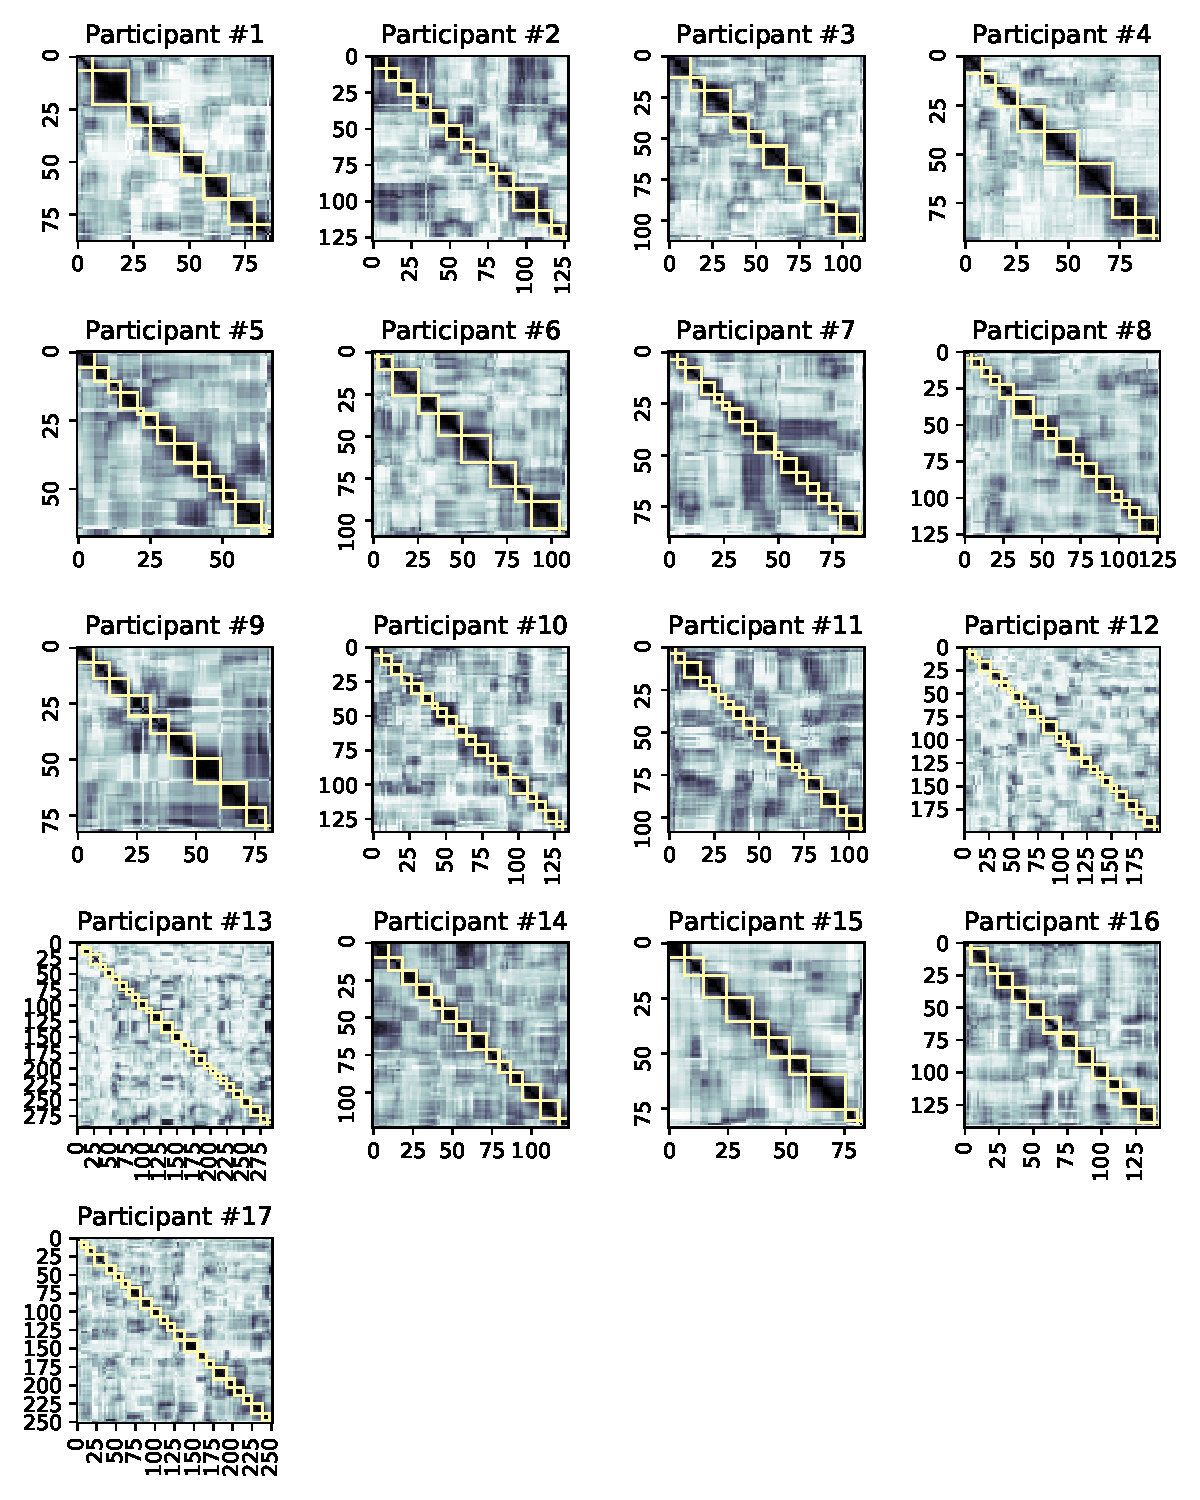
\includegraphics[width=1\textwidth]{figs/supp1_corrmats.pdf}
\caption{\small \textbf{Recall model correlation matrices and event segmentation fits.} Each participant's timepoint-by-timepoint recall correlation matrix.  The yellow boxes represent ``events'' identified by a hidden Markov model.}
\label{fig:corrmats}
\end{suppfigure}

\begin{suppfigure}[t!]
\centering
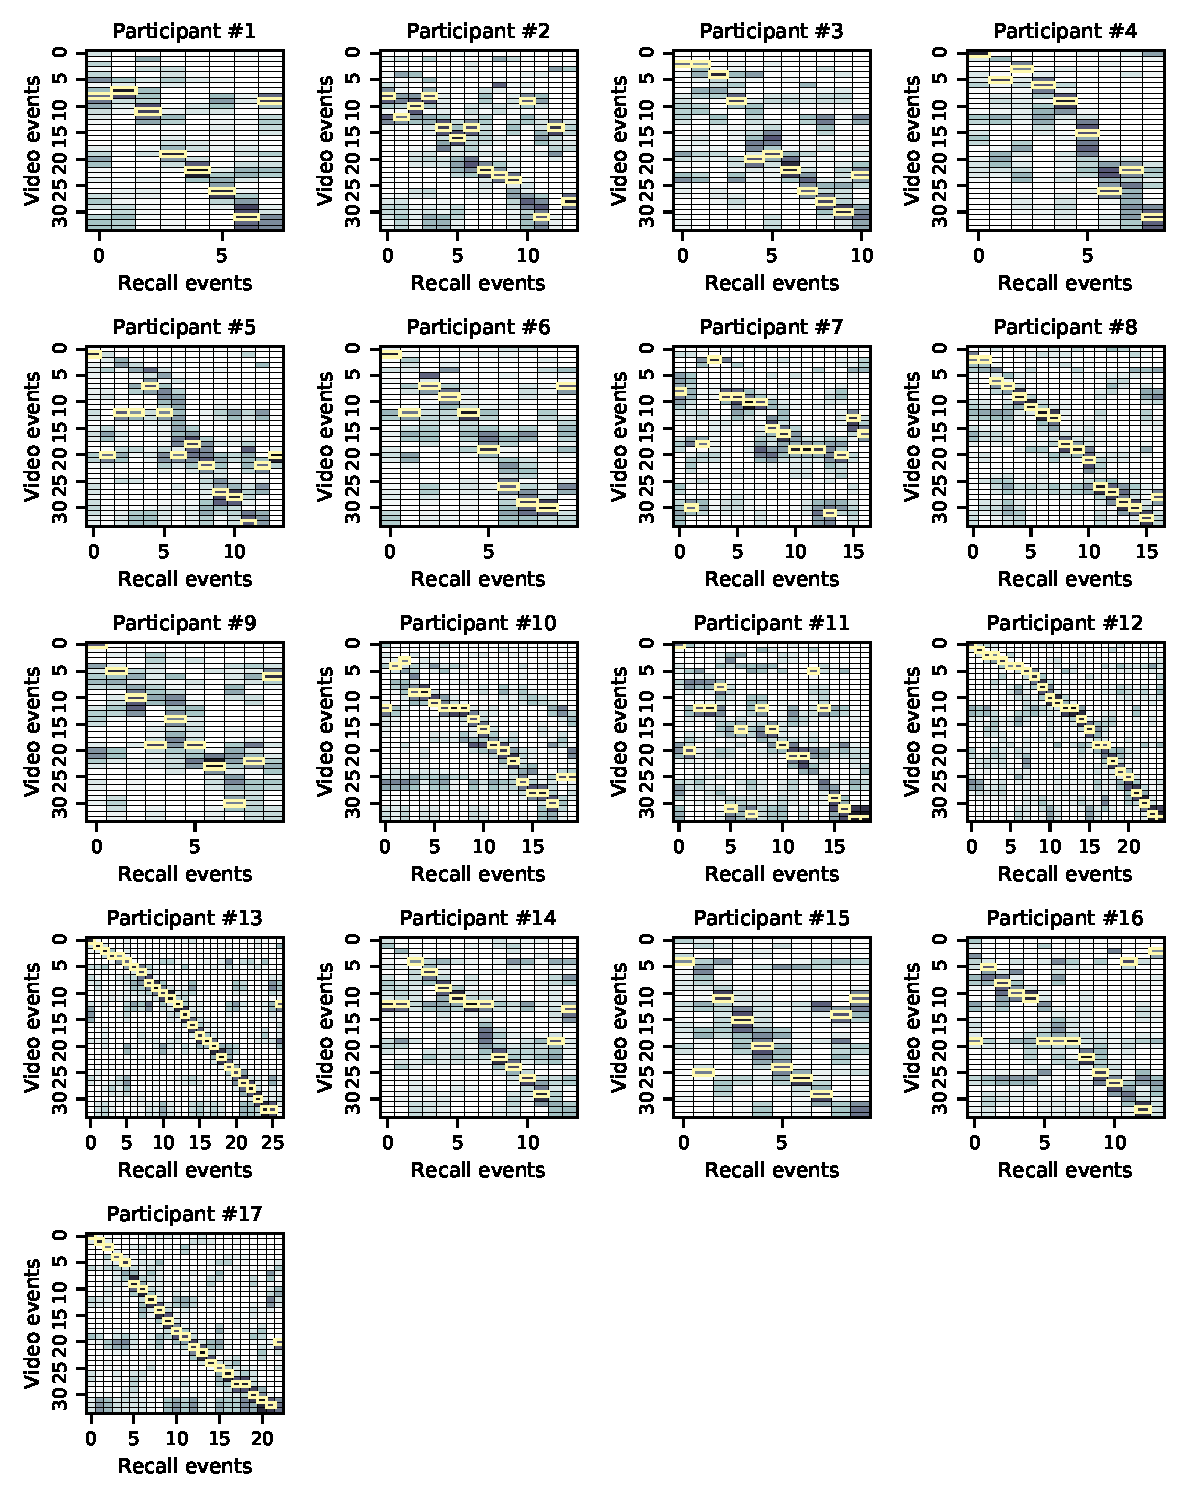
\includegraphics[width=1\textwidth]{figs/supp2_matchmats.pdf}
\caption{\small \textbf{Video-recall event model correlation matrices.} Each participant's video event by recall event correlation matrix.  The yellow boxes represent the maximum correlation in each column.}
\label{fig:matchmats}
\end{suppfigure}

\section{Additional measures of naturalistic memory}
To quantify the similarity between the video model and individual recall models, we considered a number of novel metrics.  First, we tested whether each participant's recall model matched the movie model in a general sense. To do this, for each participant we filtered the video model to only include the events that the participant remembered and computed the root mean squared difference (RMSD) between the video model and the recall model. As an example, if the participant remembered all the events in order (with perfect precision), the expected distance value would be 0. However, if they remembered a subset of events, events our of order or with low precision the expected distance would be greater than 0. To assess significance, we performed a permutation test where we circularly shifted the recall model (10000 times) and recomputed the RMSD. The recall model significantly matched the video model for nine of the participants ($p$<.05, permutation test, see Methods for details; participants: 3-4, 8-13, 17 and the p-value for the rest of the participants was less than .25). Furthermore, the RMSD values were significantly correlated to hand annotated memory performance across participants (Pearson's $r$(16)=-.57, $p$=.016). Thus, a closer match between the video and recall event models was related to better recall performance.

Next, we tested whether participants who recalled more events were also more precise in their recollections. For each participant, we computed the correlation between each recall event and its matching video event (only for the events which they recalled). This resulted in a single number for each recalled event indexing how similar the recall event was to its matching movie event (i.e the ``precision'' of the recall). We then averaged the correlations within participant. In line with our prediction, there was a strong correlation between hand annotated memory performance and precision suggesting that participants who remembered more events also remembered them more veridically (Pearson's $r$(16)=.74, $p$=.0006). Then, we considered the distinctiveness of each recall event. That is, how uniquely a recall event matched a given video event compared to all other video events. We hypothesized that participants with high memory performance might describe each event in a more distinctive way (relative to those with lower memory performance who might describe events in a more general way). To this end, we computed a `distinctiveness' score for each participant (i.e. 1 - the correlation between a recall event and all non-matching video events).  Then, we averaged this measure over recall events within participant.  We found that participants with higher hand annotated memory performance also had higher distinctiveness scores (Pearson's $r$(16)=.8, $p$=.0001).

Lastly, we tested whether participants with better memory performance were also more likely to remember the events in order.  For each participant, we computed the Spearman rank correlation between the order of events that the participant recalled and the actual order of events (filtering events that were actually recalled).  We found that participants who recalled more events also recalled more of them in order (Pearson's $r$(16)=.5, $p$=.04). In summary, we found that better memory performance was associated with more precise, distinctive and ordered recalls.

\section{Naturalistic extensions of classic list-learning analyses}
Just like in a traditional ``free-recall'' list-learning experiment where participants view a list of words and then verbally recall them, our video-recall matching analysis approach affords us the ability to analyze memory in the same way. The recalled events can be treated as ``items'' analogous to words recalled in a list-learning study. In our first set of analyses, we sought to characterize memory performance/dynamics by extending classic analyses originally designed for list-learning experiments to more naturalistic settings. First, we asked whether the estimated number of recall events ($k$) by participant was related to hand-annotated accuracy as published in Chen et al. (2017).  We found a strong positive correlation where subjects with a greater number of recall events also had better overall memory performance (Pearson's $r$(16)=.67, $p$=.003). Then, we considered how participants initiated the recall sequence (known in the literature as the `probability of first recall' or `PFR'). We found that participants tended to initiate their recall sequences with the first few events (Supp. Fig.~\ref{fig:list-learning}a), which is qualitatively very similar to previously published list learning experiments (REF?). Next, we considered another well-studied memory measure in the list-learning literature, the lag conditional response probability curve (or lag-CRP) ~\citep{Kaha96}. The result suggests a strong bias to transition sequentially events in the forward direction (Supp. Fig.~\ref{fig:list-learning}b). Finally, we assessed memory performance for each event in the video as a function of its serial position during encoding (Supp. Fig.~\ref{fig:list-learning}c). We found that there was substantial variability in memory for the different events (STAT). We also considered two additional across-participant measures of recall that characterize memory organization: temporal clustering and semantic clustering. We found that participants who clustered in time also recalled a greater number of events (Pearson's $r$(16)=.62, $p$=.007). Next, we assessed semantic clustering. We found that the semantic clustering score was related to memory performance across participants (Pearson's $r$(16)=.55, $p$=.02).  Thus, participants who organized their recalls with respect to the semantic information contained in the scene had better memory performance.


\begin{suppfigure}[t!]
\centering
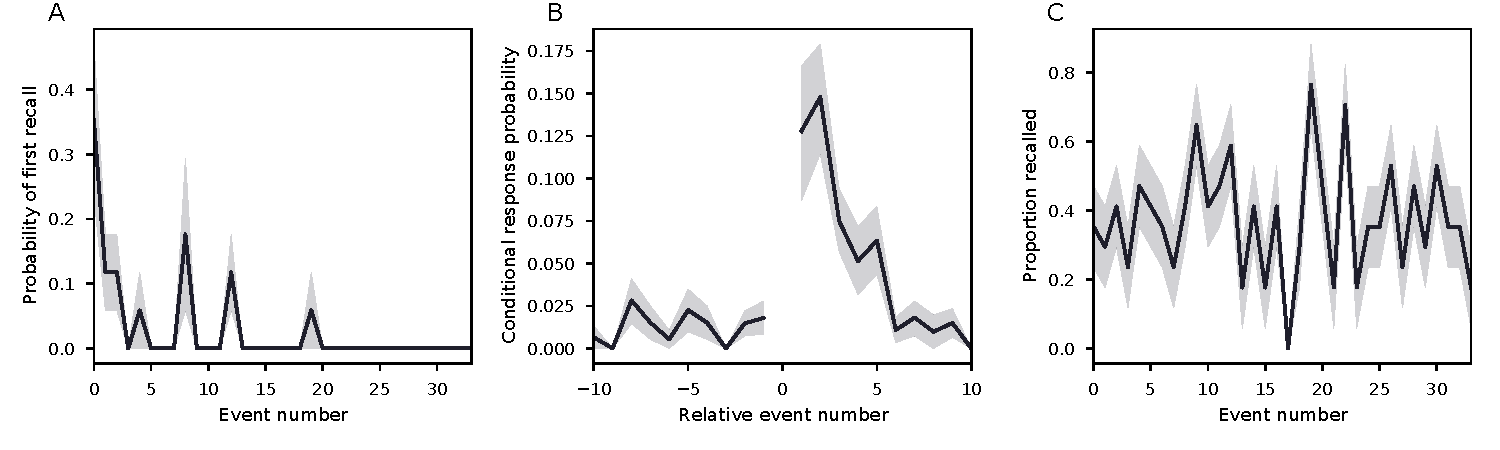
\includegraphics[width=1\textwidth]{figs/supp3_list_learning.pdf}
\caption{\small \textbf{Naturalistic extensions of classic list-learning memory analyses.} A). The probability of first recall as a function of the serial position of the event during encoding. B). A lag-conditional response probability curve. Given recall of event i, the probability that the next recalled item will be from serial position i +/- lag. C). Proportion of events recalled as a function of serial position. All error bars are the standard error of the mean derived from a bootstrap resampling procedure.}
\label{fig:list-learning}
\end{suppfigure}

\section{Supplemental Methods}

\subsection{Characterizing memory performance using traditional approaches}
\textbf{Overall Accuracy.}  To get an overall measure of the quantity of information recalled, we computed the proportion of sucessfully recalled events by counting the number of unique recall events identified by the HMM model and dividing by the total number of video events.  We performed this analysis for each participant separately.

\textbf{Probability of first recall (PFR).}  The (PFR) analysis represents the probability that an item will be recalled first as a function of its serial position during encoding. We initialized a \# of participants (17) by \# of video events (34) matrix. Then for each participant, we found the index of the video event that was recalled first and filled in that index in the matrix with a 1.  Finally, we averaged over the rows of the matrix, resulting in a 1 by 34 array representing the proportion of subject that recalled an event as a function of serial position during encoding.

\textbf{Lag conditional probability curve (lag-CRP).} The lag-CRP represents the probability that the next item recalled will be of lag $i$ from the just recalled item. For each recall transition, we computed the lag between the current recall event and the next recall event, normalizing by the total number of possible transitions.  This resulted in a \# of participants (17) by lags (-33:+33) matrix. We averaged over the rows of this matrix to get a group-averaged lag-CRP.

\textbf{Serial position curve (SPC).} The SPC represents the proportion of participants that remember an item as a function of its serial position during encoding. We initialized a \# of participants (17) by \# of video events (34) matrix. Then, for each recall event (and each participant), we found the index of the video event that was recalled and filled it in with a 1. This resulted in a matrix where 1s indicate the successful recall of an event in serial position $n$ and zeros indicate the lack of recall for that event.  Lastly, we averaged over the rows of the matrix to get a 1 by 34 array representing the proportion of subjects that recalled an event as a function of its serial position.

\textbf{Temporal clustering.} Temporal clustering measures the extent to which participants group their recall responses according to encoding position ~\citep{PolyEtal09}. For instance, if the participant recalled each item in the presentation order, this would result in a score of 1. If the participant recalled randomly with respect to presentation order, this would result in a score of ~.5.  For each event transition (and separately for each participant), we computed the rank similarity (euclidean distance) between the presentation position  of the current and next recall events. The scores were then averaged within participant to get a single number representing the extent of temporal clustering exhibited by a given participant.

\textbf{Semantic clustering.} Similar to temporal clustering, semantic clustering measures the extent to which participants group their recall responses according to semantic similarity ~\citep{PolyEtal09}. Here, we are using the topic vectors for each event as a proxy for its semantic content. Thus, similarity between the semantic content for two events can be computed by correlating their respective topic vectors.  For instance, if each consecutive recall was the next most similar event (in terms of its s), this would result in a score of ~1. If the participant recalled randomly with respect to semantic similarity, this would result in a score of ~.5.  For each event transition (and separately for each participant), we computed the rank similarity (correlation distance) between the current recall event and the next recall event. The scores were then averaged within participant to get a single number representing the extent of semantic clustering exhibited by a given participant.

\end{document}
